\documentclass[11pt]{article}

\usepackage[final]{acl}
\usepackage{times}
\usepackage{latexsym}
\usepackage{url}
\usepackage[T1]{fontenc}
\usepackage[utf8]{inputenc}
\usepackage{microtype}
\usepackage{inconsolata}

\usepackage{graphicx}
\usepackage{booktabs}
\usepackage{multirow}
\usepackage{array}
\usepackage{amsmath}
\usepackage{float}

\title{Comparative Analysis of Retrieval-Augmented Generation Architectures for Financial Question Answering}

\author{Uday Jain \\
  Department of Statistics and Machine Learning \\
  Linköping University, Linköping, Sweden 581 83 \\
  \texttt{udaja983@student.liu.se} }

\date{}

\begin{document}
\maketitle

\begin{abstract}
This study evaluates five Retrieval-Augmented Generation (RAG) architectures for 
financial QA using the FiQA dataset. We compare Naive RAG, Re-Ranking RAG, 
Hypothetical Document Embeddings (HyDE), Query Expansion RAG, and Multi-Step 
Iterative RAG across lexical, semantic, and retrieval metrics. Results show 
Re-Ranking RAG achieves best lexical performance (8\% higher ROUGE-L, 177\% 
higher BLEU vs Naive) but with higher variability. Naive RAG provides superior 
semantic preservation (5\% higher cosine similarity) and consistency. Retrieval 
quality shows limited correlation with generation performance (r<0.30), 
challenging RAG design assumptions.
\end{abstract}


\section{Introduction}

Retrieval-Augmented Generation (RAG) has emerged as a dominant paradigm for 
knowledge-intensive natural language tasks, combining the strengths of 
information retrieval and large language models. While the basic RAG 
architecture is well-established, numerous advanced variants have been proposed 
to address limitations in retrieval quality, relevance, and answer coherence. 
However, there remains a lack of systematic comparative evaluation of these 
architectures, particularly in highly specialised and technical domains such as 
financial question answering, where precise terminology and factual accuracy are critical.

Financial domain QA presents unique challenges (1) Terminology specificity: 
Domain-specific jargon requires precise retrieval (2) Factual precision: Incorrect 
financial information can have serious consequences (3) Regulatory compliance: 
Answers must align with established financial principles (4) Multi-faceted 
queries: Often combine quantitative and qualitative aspects. This study addresses 
this gap by implementing and evaluating five RAG architectures.

Using the FiQA financial dataset \citep{maia2018fiqa}, we conduct a comprehensive 
evaluation across \textbf{12 complementary metrics} spanning lexical, semantic, 
and retrieval dimensions to answer three research questions:

\begin{enumerate}
    \item How do advanced RAG architectures compare to the naive baseline in 
    financial QA, particularly regarding domain-specific terminology handling?
    \item What is the relationship between retrieval quality metrics and final 
    generation quality across different architectures?
    \item Which evaluation metrics provide the most discriminative power for 
    architecture comparison in financial domains?
\end{enumerate}

Our contributions include: (1) Implementation framework: Open-source modular 
framework for RAG architecture experimentation (2) Empirical evidence: 
Comprehensive benchmarking providing architecture selection guidance for 
financial QA (3) Metric insights: Analysis of which evaluation metrics best 
capture architectural differences in specialised domains (4) Domain-specific 
findings: Identification of architecture behaviours specific to financial 
terminology and precision requirements

\section{Theoretical Background}

\subsection{Retrieval-Augmented Generation}
The RAG framework \citep{lewis2020rag} combines a retrieval component $R(q)$ 
that retrieves relevant documents $D$ for query $q$, and a generation component 
$G(q, D)$ that produces an answer conditioned on both the query and retrieved 
documents: $Answer = G(q, R(q))$

This architecture addresses two key limitations of pure LLMs: (1) reliance on 
parametric knowledge that may be outdated or incomplete, and (2) hallucination 
when generating facts not in training data. By grounding generation in retrieved 
evidence, RAG improves factuality and allows access to current information.

\subsection{Advanced RAG Architectures}

\paragraph{Re-Ranking RAG} employs a two-stage retrieval process: initial 
retrieval using dense embeddings followed by re-ranking with a cross-encoder 
model \citep{nogueira2019multi}. This addresses the \textit{double penalty} 
problem where semantically relevant but lexically different documents are 
missed by single-stage retrieval. The final relevance score combines both stages:
$s_{\text{final}} = \alpha \cdot s_{\text{dense}} + (1-\alpha) \cdot s_{\text{cross}}$

where $s_{\text{dense}}$ represents cosine similarity from dense retrieval and 
$s_{\text{cross}}$ represents relevance probability from the cross-encoder.

\paragraph{Hypothetical Document Embeddings (HyDE)} \citep{gao2023hyde} 
generates a hypothetical answer to the query using the LLM, then uses this 
as the retrieval query. This approach bridges the \textit{lexical gap} between 
user queries and relevant documents by mapping from query space to answer space:
$q_{\text{hyde}} = \text{LLM}(q_{\text{original}})$

The intuition is that the hypothetical answer shares more lexical and semantic 
similarity with relevant documents than the original query.

\paragraph{Query Expansion RAG} generates multiple query variations to address 
vocabulary mismatch and increase retrieval recall \citep{zhuang2023query}. 
Given original query $q$, the system generates $n$ expansions $\{q_1, q_2, ..., q_n\}$:
$R_{\text{expanded}}(q) = \bigcup_{i=1}^{n} R(q_i)$ The union of retrieved 
documents from all expansions provides broader coverage, particularly valuable 
for technical domains where terminology may vary.

\paragraph{Multi-Step Iterative RAG} employs an iterative retrieval process 
where intermediate answers inform subsequent retrieval steps \citep{jiang2023retrieval},
mimicking human reasoning in complex QA through query refinement based on 
intermediate answers.

\subsection{Evaluation Framework}
We employ a multi-faceted evaluation approach addressing different quality dimensions:

\begin{itemize}
    \item \textbf{Lexical Metrics}: ROUGE-1/2/L/LSum \citep{lin2004rouge} measure 
    n-gram overlap. ROUGE-1 (unigrams) captures content coverage, ROUGE-2 
    (bigrams) assesses phrase structure, while ROUGE-L (Longest Common Subsequence) 
    evaluates sentence-level similarity.
    
    \item \textbf{Semantic Metrics}: BERTScore \citep{zhang2019bertscore} computes 
    similarity using contextual BERT embeddings, with precision (how much of 
    generated content is relevant), recall (how much of reference content is 
    covered), and F1 (harmonic mean).
    
    \item \textbf{Fluency Metrics}: BLEU score \citep{papineni2002bleu} evaluates 
    word choice and sentence structure quality, particularly important for 
    domain-specific terminology usage.
    
    \item \textbf{Embedding Similarity}: Cosine similarity between answer 
    embeddings provides a holistic semantic similarity measure complementary 
    to BERTScore.
    
    \item \textbf{Retrieval Quality}: Average retrieval score indicates 
    retrieval confidence, while retrieval similarity to ground truth context 
    measures relevance accuracy.
\end{itemize}

This comprehensive framework allows us to assess not only \textit{what} is said 
(lexical/semantic content) but also \textit{how well} it is said (fluency) and 
\textit{how} it was derived (retrieval quality).

\section{Data and Methodology}

\subsection{Dataset}
We use the FiQA dataset \citep{maia2018fiqa}, a financial question answering 
corpus via hugging face containing 57,638 documents to search for retrieval 
followed by 30 question-answer pairs with optimal retrieved contexts. 

\subsection{Implementation Details}
All architectures share common components: (1) Embedding Model(all-MiniLM-L6-v2 
384 dimensions) (2) Vector Database (Qdrant; cosine similarity indexing) (3) LLM
(Local 2.7B param microsoft/phi-2 endpoint) (4) Reranker(cross-encoder/ms-marco-MiniLM-L-6-v2)

\subsection{Parameter Optimization}
Each architecture was optimized through grid search. Naive RAG($k \in \{1,2,3,4,5\}$, 
optimal at k=4. See \ref{fig:app:naiveRag}), Re-Ranking (k=4, rerank_k=20, 
$\alpha$=0.7. See \ref{fig:app:ReRankingRagK}, \ref{fig:app:ReRankingRagRRK}), 
HyDE(k=4, temperature=0.3. See \ref{fig:app:hydeRag}), Query Expansion(k=2, 
numExpansions=4. See\ref{fig:app:qeRag},\ref{fig:app:qeRagQE}) and Multi-Step(k=2, 
kStep=3, nSteps=2. See\ref{fig:app:msikRag},\ref{fig:app:msikstepRag},\ref{fig:app:msikstepsizeRag}).

\subsection{Evaluation Protocol}
Each query was processed through all five architectures, with answers evaluated 
against ground truth using our 12-metric framework. Given the exploratory nature
of this study and the computational constraints of running statistical tests 
across 12 metrics × 5 architectures × 30 queries, we focus on descriptive 
statistics. 

\section{Results}

\subsection{Overall Performance Comparison}

Figure \ref{fig:compareOutput} presents the mean scores with standard error 
bars for each architecture across all metrics. The visual comparison reveals 
clear architectural trade-offs: Re-Ranking RAG excels in lexical metrics but 
with higher variability, while Naive RAG provides more consistent semantic 
preservation.

\begin{figure}[H]
    \centering
    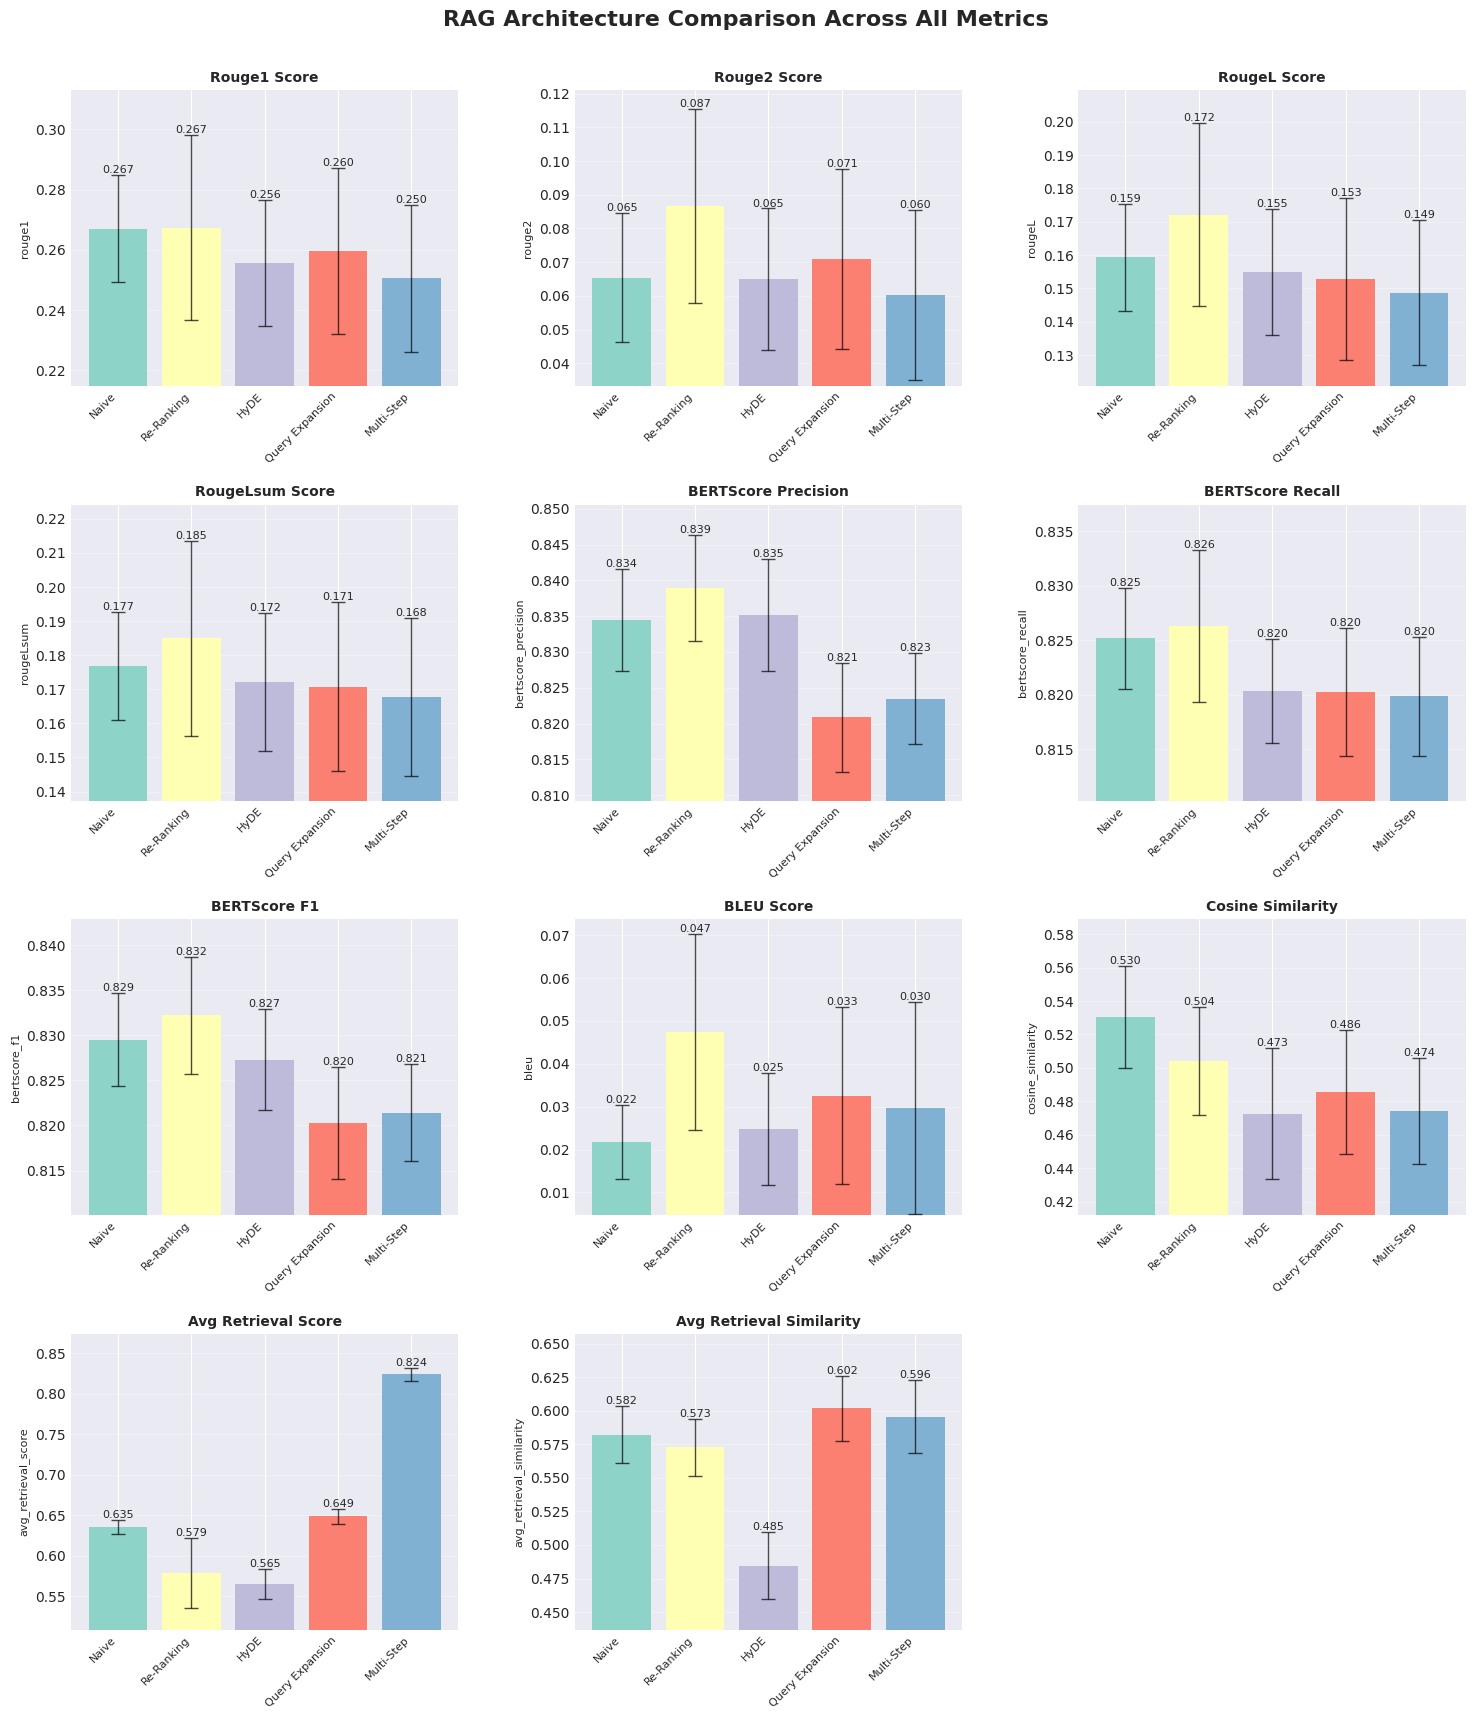
\includegraphics[width=0.35\textwidth]{images/compareOutput.png}
    \caption{Comparative analysis of RAG architectures across evaluation metrics. 
    Error bars represent standard errors}
    \label{fig:compareOutput}
\end{figure}

\subsection{Correlation Analysis Revealing Metric Relationships}

Correlation analysis (Figure~\ref{fig:correlations}) reveals critical RAG evaluation insights:

\paragraph{Metric Redundancy} Near-perfect ROUGE inter-correlations (ROUGE-L vs LSum: r=0.98) make reporting multiple variants redundant. Strong BLEU-ROUGE correlation (r=0.91) indicates overlapping constructs.

\paragraph{Retrieval-Generation Independence} Weak correlations (r<0.30) support separate evaluation. Retrieval similarity correlates moderately with semantic metrics (r=0.49) but negligibly with lexical metrics.

\paragraph{Practical Recommendations} We recommend: ROUGE-L (lexical), Cosine + BERTScore F1 (semantic), BLEU (fluency), and retrieval similarity only. This reduces 12 to 5 metrics while maintaining coverage.

\begin{figure}[H]
    \centering
    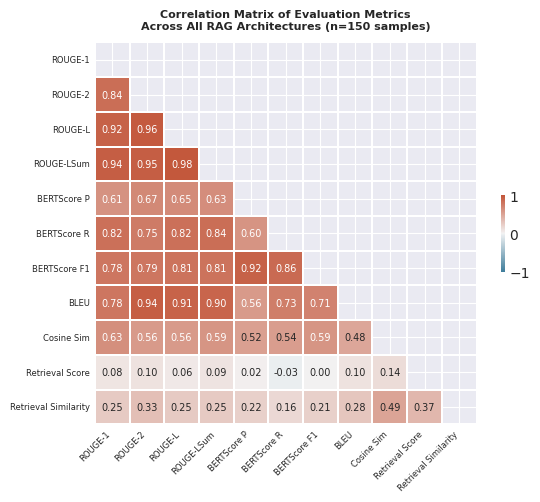
\includegraphics[width=0.35\textwidth]{images/correMatrix.png}
    \caption{Correlation matrix between evaluation metrics across all 
    architectures (n=150 samples)}
    \label{fig:correlations}
\end{figure}

\subsection{Key Observations}

\paragraph{Lexical Performance with Variability} Re-Ranking RAG outperforms 
all other architectures across all ROUGE metrics (ROUGE-L: 0.172 vs 0.159 
for Naive, \textbf{8\% relative improvement}). However, this comes with 
substantially higher standard errors (ROUGE-L SE: 0.027 vs 0.016 for Naive), 
indicating greater response inconsistency. This suggests that while 
cross-encoder re-ranking can significantly improve lexical alignment, 
its effectiveness varies across queries.

\paragraph{Semantic Preservation in Simpler Architectures} Despite lower 
lexical scores, Naive RAG maintains superior cosine similarity (0.530 vs 
0.504 for Re-Ranking, \textbf{5\% higher}) and competitive BERTScore metrics 
(F1: 0.829 vs 0.832 for Re-Ranking). Coupled with the lowest standard errors 
across metrics, this indicates that simpler architectures provide more 
reliable semantic preservation, albeit with less lexical precision.

\paragraph{Fluency as Key Discriminator} BLEU scores show the largest 
architectural differences, with Re-Ranking outperforming Naive by 
\textbf{177\%} (0.047 vs 0.021). This substantial gap suggests that 
re-ranking significantly improves word choice and sentence structure 
fluency, making BLEU a particularly sensitive metric for architecture 
comparison in financial QA.

\paragraph{Retrieval-Generation Decoupling} Despite having the lowest 
average retrieval score (0.578 vs 0.635 for Naive, \textbf{9\% lower}), 
Re-Ranking produces the best answers. This counterintuitive finding 
suggests that retrieval confidence metrics may not correlate with 
generation quality, possibly because high-confidence retrievals lack 
the diversity needed for comprehensive answers and because of smaller LLM.

\paragraph{HyDE's Domain-Specific Underperformance}: HyDE shows 
the poorest retrieval similarity (0.485 vs 0.582 for Naive, 
\textbf{17\% lower}), suggesting that hypothetical document generation 
struggles with financial domain precision. This performance appears 
highly dependent on the LLM's ability to generate accurate hypothetical 
financial content.

\paragraph{Query Expansion's Limited Impact}: Despite generating 
multiple query variations, Query Expansion showed limited improvements over 
Naive RAG (ROUGE-L: 0.153 vs 0.159, \textbf{4\% lower}) and reduced cosine 
similarity (0.486 vs 0.530, \textbf{9\% lower}). This suggests that query 
expansion alone, without corresponding refinement mechanisms, provides 
limited benefit.
\paragraph{Multi-Step's Retrieval-Quality Mismatch}: Multi-Step 
achieves the highest retrieval similarity (0.596) and exceptionally 
high average retrieval score (0.824), but this doesn't translate to 
generation quality (lowest ROUGE scores: 0.149 vs 0.172 for Re-Ranking). 
The high retrieval scores with similar documents suggest limited 
diversity and the iterative process appears constrained by LLM 
performance bottlenecks.
\end{itemize}

\section{Discussion}

\subsection{Interpretation of Architectural Trade-offs}

The superior lexical performance of Re-Ranking RAG can be attributed to its 
dual-stage retrieval process supports the theoretical advantage of cross-encoder 
refinement for domain-specific retrieval. In financial contexts where precise 
terminology matters (e.g., distinguishing between "401(k)" retirement plans and 
general investment options), the semantic understanding of cross-encoders 
appears particularly valuable. However, the observed variability (standard errors 
72\% higher than Naive RAG for ROUGE metrics) suggests this advantage is 
query-dependent or inherently cross-encoders dependent, recommending use of 
domain specific trained cross-encoders where domain specific relevance takes 
precedence over semantic similarity.

The strong semantic performance of Naive RAG despite poor BLEU scores suggests 
a trade-off: simpler architectures may preserve semantic meaning but struggle 
with fluency and structure. This aligns with findings by \citet{lewis2020rag} 
that retrieval quality doesn't linearly translate to generation quality.
Comparable overall performance coupled with a strong consistency also presents a 
compelling case for simpler architectures in production systems unless custom 
domain trained embeddings are used. The minimal performance 
gap in BERTScore metrics (≤0.003 difference in F1) coupled with significantly 
lower standard errors suggests that for many financial QA applications, the 
additional complexity of advanced architectures may not justify their 
computational cost unless coupled with custom trained models on domain specific 
data.

\subsection{The BLEU Metric as Architectural Discriminator}

The dramatic BLEU score differences (177\% improvement for Re-Ranking) highlight 
this metric's sensitivity to architectural improvements in financial QA. Unlike 
general domains where BLEU may penalize legitimate paraphrasing, in financial 
contexts where precise terminology is crucial, BLEU effectively captures 
architecture's ability to generate fluent, domain-appropriate language. This 
makes BLEU particularly valuable for architecture comparison in technical domains.

\subsection{Retrieval Quality Misalignment}

The inverse relationship between retrieval confidence metrics and generation 
quality challenges conventional assumptions about RAG system design. Our 
findings suggest that:
\begin{enumerate}
    \item High retrieval similarity scores may indicate \textit{overfitting} 
    to a narrow set of documents, limiting answer comprehensiveness
    \item Moderate-confidence retrievals with higher diversity better 
    support the LLM's generation capabilities
    \item Current retrieval metrics may need augmentation with diversity 
    measures to better predict generation quality
\end{enumerate}

\subsection{Limitations and Methodological Considerations}

Study limitations contextualize findings:
\begin{enumerate}
    \item \textbf{Single-domain evaluation}: Financial QA characteristics may not generalize
    \item \textbf{LLM constraints}: Single 2.7B parameter model limits generalizability
    \item \textbf{Statistical analysis}: Descriptive patterns without formal hypothesis testing
    \item \textbf{Computational scope}: 30 queries may represent limited variability
\end{enumerate}

Despite limitations, performance magnitude and consistent patterns provide 
meaningful architecture selection insights.

\subsection{Related Work in RAG Evaluation}
Systematic architectural RAG comparisons remain limited. Our HyDE results align 
with \citet{gao2023hyde}'s variable performance findings, though we use a technical 
domain dataset versus general ones. Re-Ranking success supports \citet{nogueira2019multi}'s 
cross-encoder effectiveness. \citet{zhuang2023query} demonstrated query expansion in 
web search but not specifically for RAG. \citet{jiang2023retrieval} proposed iterative 
retrieval without comprehensive benchmarking. Our study addresses this gap through 
systematic five-architecture comparison in financial QA with domain-specific 
multi-metric evaluation.

\subsection{Qualitative Analysis}
Manual inspection of samples revealed Re-Ranking's precise terminology and 
source citation, Naive's verbosity with semantic correctness, HyDE's occasional 
hallucinations, Query Expansion's broader concept coverage, and Multi-Step's 
document redundancy due to LLM bottlenecks.

\subsection{Reproducibility}
Our complete implementation is available at: \url{https://github.com/SpikeStriker/732A81_text_mining_research_project/tree/main/EvaluatingRagArchitecture}. 

\section{Conclusion}

This study provides empirical evidence for RAG architecture selection in 
financial question answering through comprehensive evaluation across five 
architectures and twelve metrics. Our key findings reveal important 
trade-offs and considerations:

\begin{enumerate}
    \item \textbf{Performance-Variability Trade-off}: Re-Ranking RAG offers 
    superior lexical performance and fluency but with higher response variability, 
    while Naive RAG provides more consistent semantic preservation with 
    competitive performance.
    
    \item \textbf{Metric Sensitivities}: Different metrics reveal distinct 
    architectural strengths—BLEU best captures fluency improvements, 
    ROUGE identifies lexical precision, while cosine similarity highlights 
    semantic preservation.
    
    \item \textbf{Retrieval-Generation Decoupling}: Retrieval quality 
    metrics show limited correlation with generation quality, suggesting 
    that current retrieval evaluation may not adequately predict final 
    answer quality.
    
    \item \textbf{Domain-Specific Architecture Suitability}: In financial 
    QA where precise terminology is critical, Re-Ranking's cross-encoder 
    refinement provides clear advantages, though simpler architectures 
    remain competitive for semantic-focused applications.
\end{enumerate}

These findings have practical implications for RAG system design in 
specialized domains: architects must balance the precision benefits of 
advanced techniques against their computational costs and variability. 
The choice ultimately depends on application priorities—precision vs 
consistency, fluency vs semantic preservation, and performance vs cost.

\subsection{Future Research Directions}

\begin{itemize}
    \item \textbf{Statistical validation}: Larger-scale studies with formal 
    hypothesis testing to confirm observed patterns
    \item \textbf{LLM impact analysis}: Systematic investigation of how different 
    LLMs (size, architecture, training) interact with RAG architectures
    \item \textbf{Dynamic architecture selection}: Developing query-based 
    heuristics for selecting optimal architectures per query type
    \item \textbf{Cross-domain evaluation}: Testing architectural patterns 
    across multiple specialized domains (legal, medical, technical)
\end{itemize}

\section*{Acknowledgments}
We thank the Text Mining course instructors for guidance and the creators of the 
FiQA dataset.

\bibliography{references}
\bibliographystyle{acl_natbib}

\appendix
\section{RAG Parameter Optimisations}
\subsection{Naive RAG}
\begin{figure}[H]
    \centering
    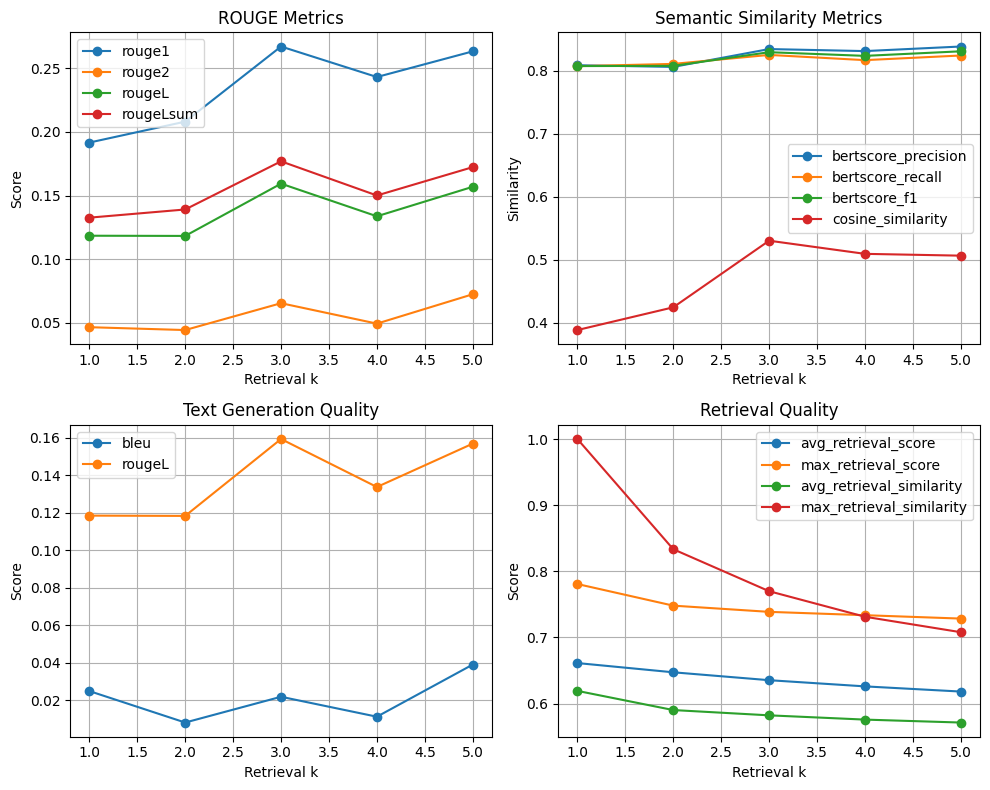
\includegraphics[width=0.5\textwidth]{images/naiveRag.png}
    \caption{Optimizing for k Retrieval}
    \label{fig:app:naiveRag}
\end{figure}

\subsection{Re-Ranking RAG}
\begin{figure}[H]
    \centering
    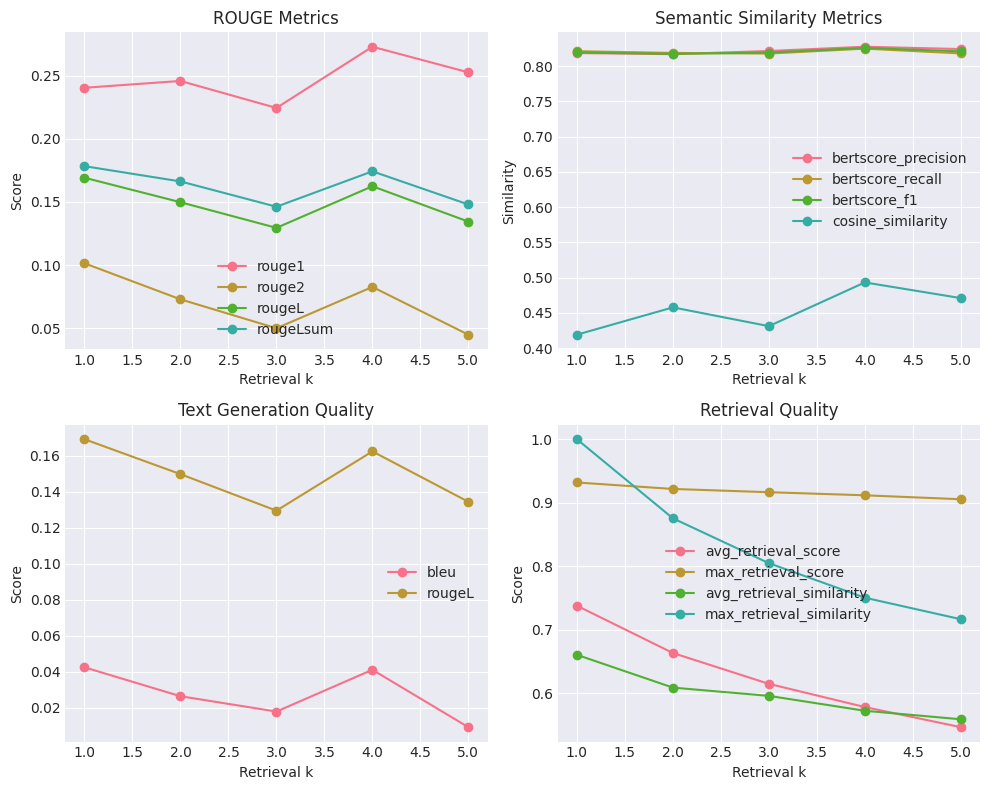
\includegraphics[width=0.5\textwidth]{images/ReRankingRagK.png}
    \caption{Optimizing for k Retrieval}
    \label{fig:app:ReRankingRagK}
\end{figure}
\begin{figure}[H]
    \centering
    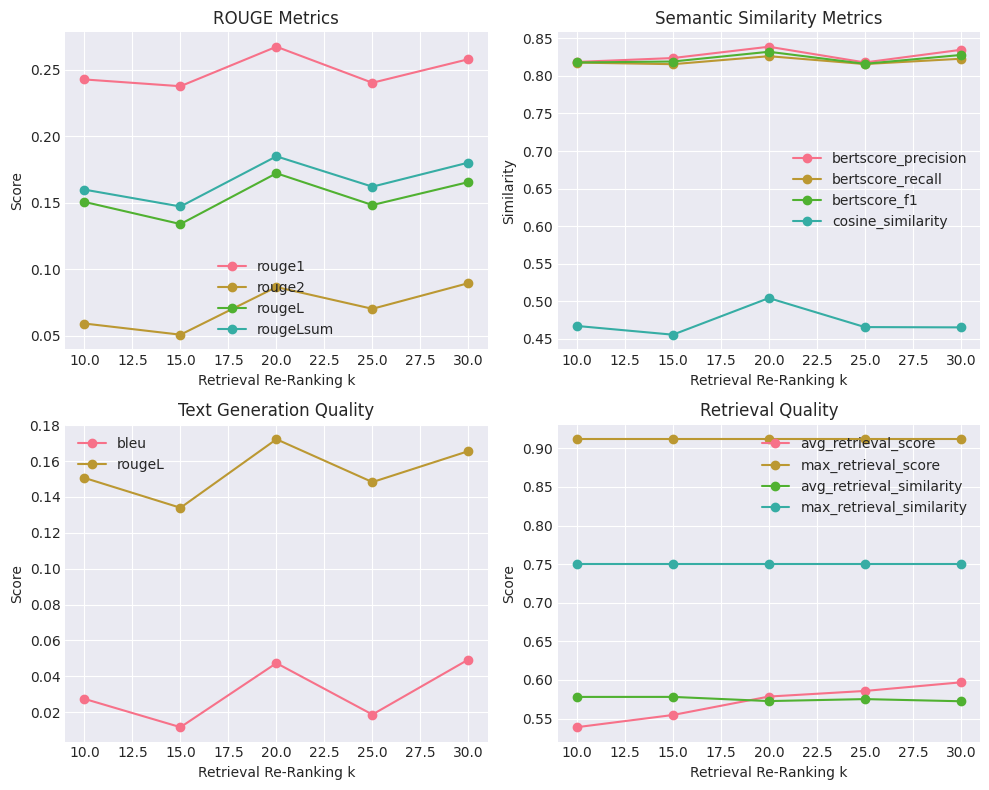
\includegraphics[width=0.5\textwidth]{images/ReRankingRagRRK.png}
    \caption{Optimizing for k Re-Ranking Retrieval}
    \label{fig:app:ReRankingRagRRK}
\end{figure}
\subsection{Hypothetical Document Extraction (HyDE) RAG}
\begin{figure}[H]
    \centering
    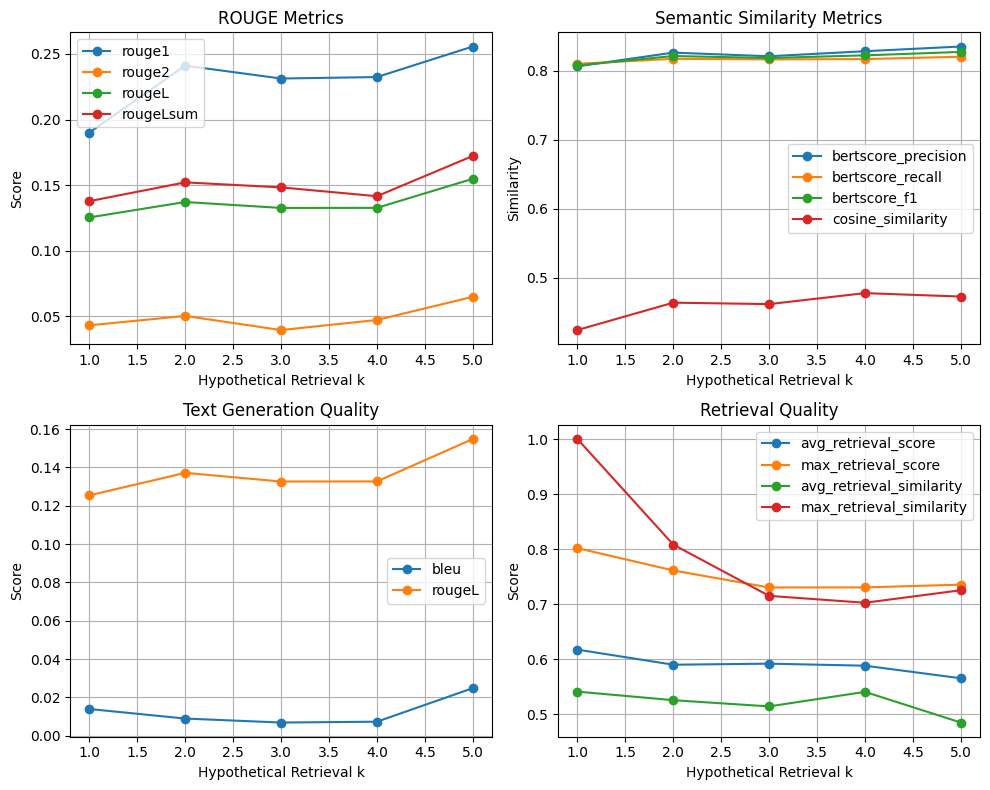
\includegraphics[width=0.5\textwidth]{images/hydeRag.png}
    \caption{Optimizing for k Retrieval}
    \label{fig:app:hydeRag}
\end{figure}
\subsection{Query Expansion RAG}
\begin{figure}[H]
    \centering
    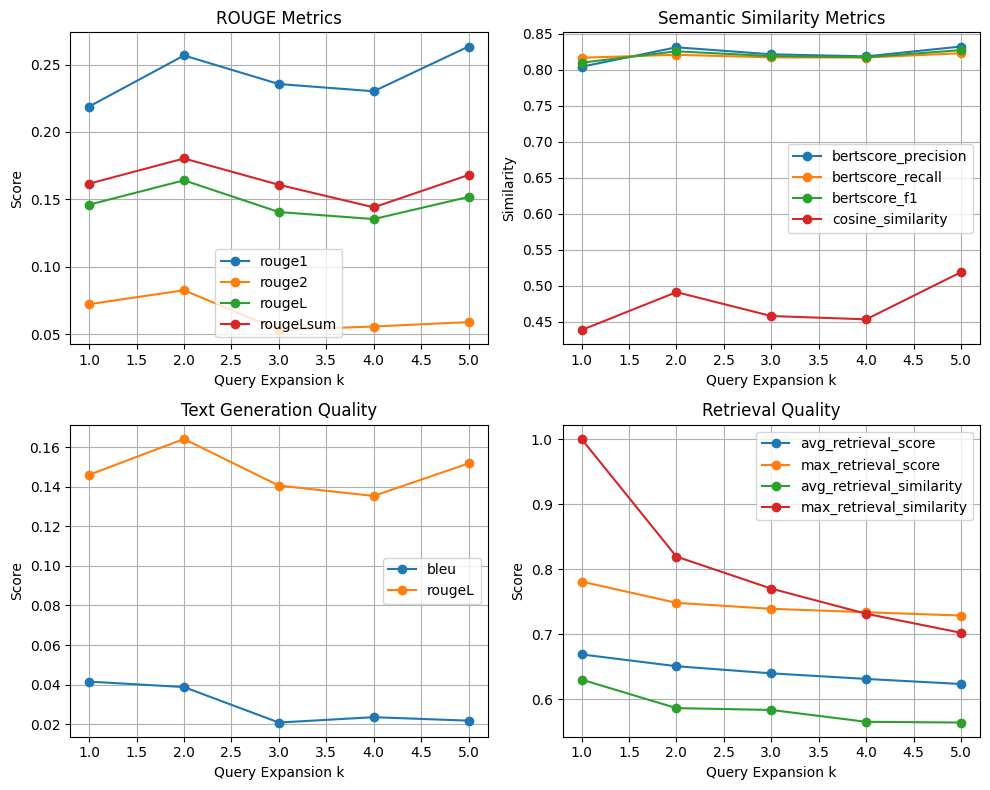
\includegraphics[width=0.5\textwidth]{images/qeRag.png}
    \caption{Optimizing for k Retrieval}
    \label{fig:app:qeRag}
\end{figure}
\begin{figure}[H]
    \centering
    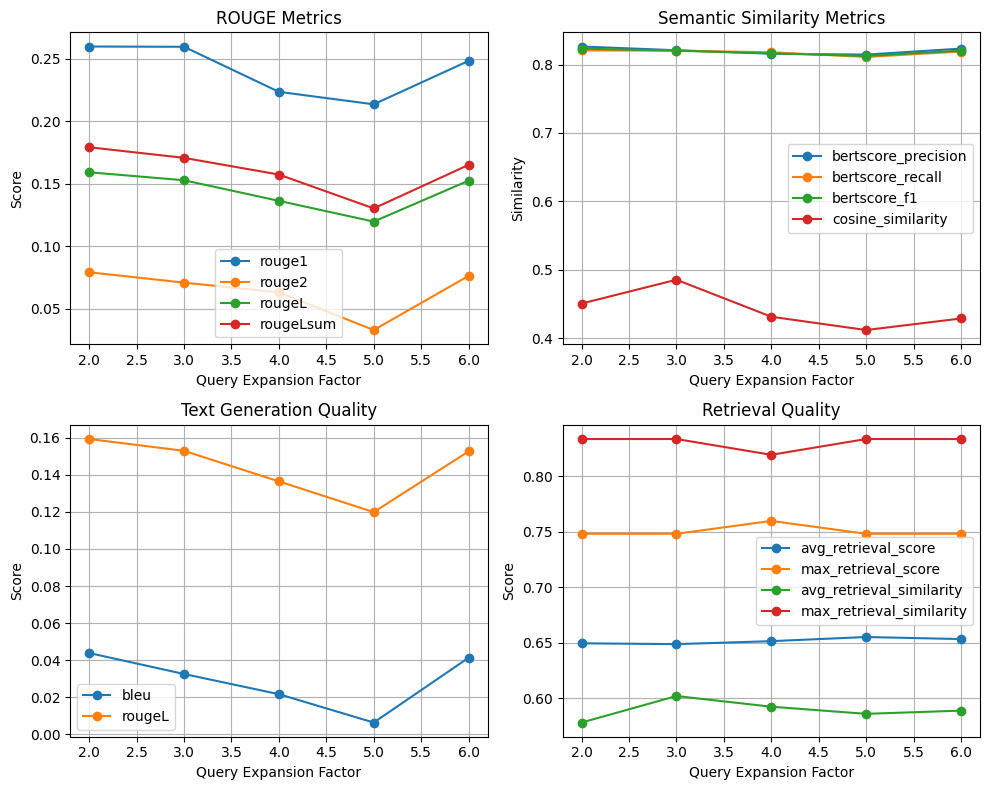
\includegraphics[width=0.5\textwidth]{images/qeRagQE.png}
    \caption{Optimizing for k Query Expansions}
    \label{fig:app:qeRagQE}
\end{figure}
\subsection{Iterative Multi-step Retrieval RAG}
\begin{figure}[H]
    \centering
    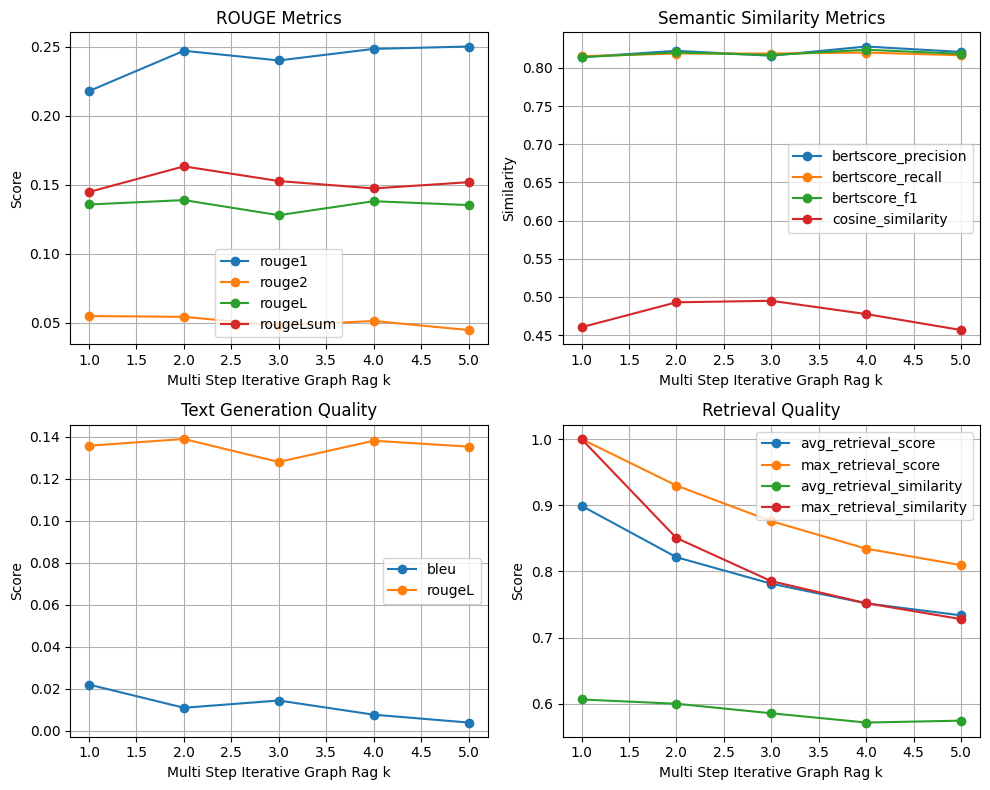
\includegraphics[width=0.5\textwidth]{images/msikRag.png}
    \caption{Optimizing for k Retrieval}
    \label{fig:app:msikRag}
\end{figure}
\begin{figure}[H]
    \centering
    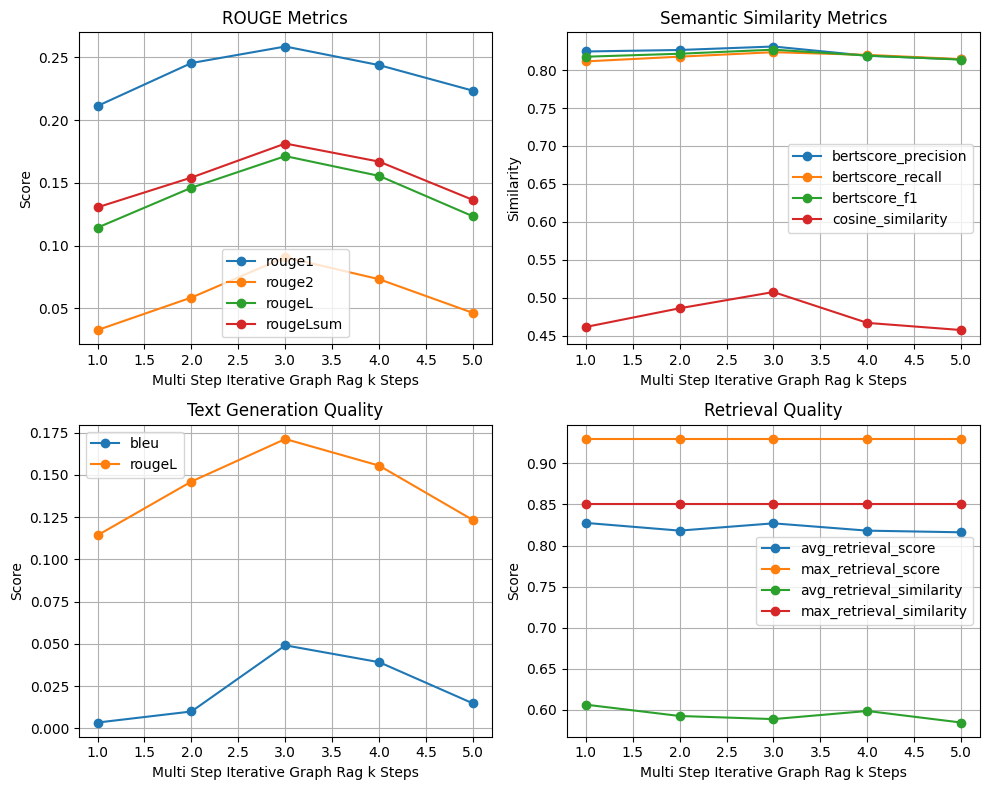
\includegraphics[width=0.5\textwidth]{images/msikstepRag.png}
    \caption{Optimizing for k iterations}
    \label{fig:app:msikstepRag}
\end{figure}
\begin{figure}[H]
    \centering
    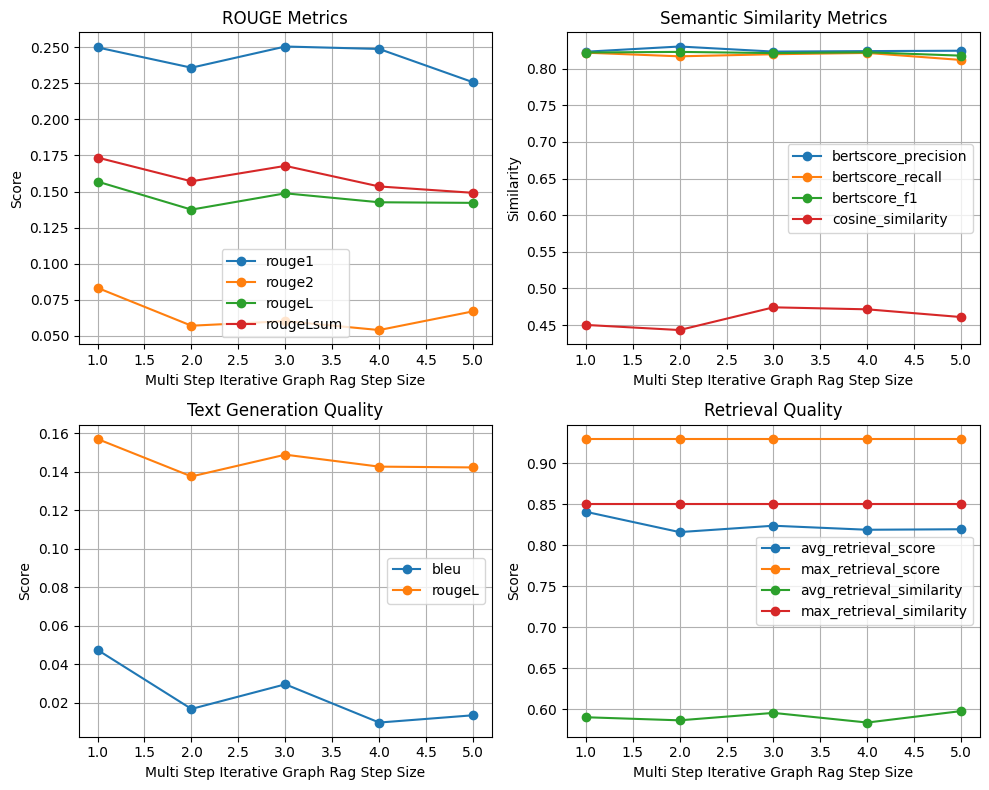
\includegraphics[width=0.5\textwidth]{images/msikstepsizeRag.png}
    \caption{Optimizing for k Retrievals in each step}
    \label{fig:app:msikstepsizeRag}
\end{figure}

\end{document}